\section{Resultados e Discussão}

Os resultados obtidos durante os dois primeiros trimestres de execução do
projeto encontram-se integralmente documentados em um repositório público
versionado, desenvolvido com o objetivo de garantir transparência,
rastreabilidade e reprodutibilidade científica das etapas computacionais
realizadas ao longo da iniciação científica \cite{leao2026vqe}.
O repositório reúne notebooks experimentais, códigos modulares em Python,
registros das simulações quânticas e dados utilizados nas etapas de
validação clássica.

A Tabela~\ref{tab:energy_comparison} apresenta uma síntese comparativa
entre as energias obtidas via VQE e os valores de referência calculados
por diagonalização exata (FCI), obtidas via implementação em Qiskit, onde $1\,E_h =1\, \text{Hartree}$ é uma unidade de energia igual ao valor absoluto da energia potencial elétrica do átomo de hidrogênio em seu estado fundamental.
\begin{table}[H]
\label{tab:energy_comparison}
\centering
\caption{Comparação entre energias obtidas via VQE e FCI. Fonte: elaboração própria (2026).}
\vspace{10pt}
\begin{tabular}{lccc}
\hline
Molécula & $E_{\text{FCI}}$ ($E_h$) & $E_{\text{VQE}}$ ($E_h$) & Erro Absoluto ($E_h$) \\
\hline
H$_2$  & $-1,8573$ & $-1,8369$ & $6,03 \times 10^{-2}$ \\
LiH    & $-8,8745$ & $-7,9576$ & $9,17 \times 10^{-1}$ \\
\hline
\end{tabular}
\end{table}



\subsection{Molécula de Hidrogênio (\texorpdfstring{H$_2$}{H2})}

Para a molécula de hidrogênio, o algoritmo VQE apresentou
comportamento de convergência consistente ao longo das iterações.
A energia variacional obtida foi
$E_{\text{VQE}} = -1,8369$ $E_h$, enquanto o valor de referência
calculado via diagonalização exata (FCI) foi
$E_{\text{FCI}} = -1,8573$ $E_h$, resultando em erro absoluto
da ordem de $6,03 \times 10^{-2}$ $E_h$, correspondente a um erro
relativo da ordem de $3\,\%$.

A Figura~\ref{fig:h2_convergence} mostra a evolução da energia ao
longo do processo de otimização. Observa-se que, após pequenas
flutuações nas iterações iniciais — esperadas devido à exploração
do espaço variacional — a energia passa a decrescer de forma
gradual até aproximadamente a iteração 60–70, quando se torna
evidente a estabilização em torno do mínimo.

\begin{figure}[H] 
\centering 
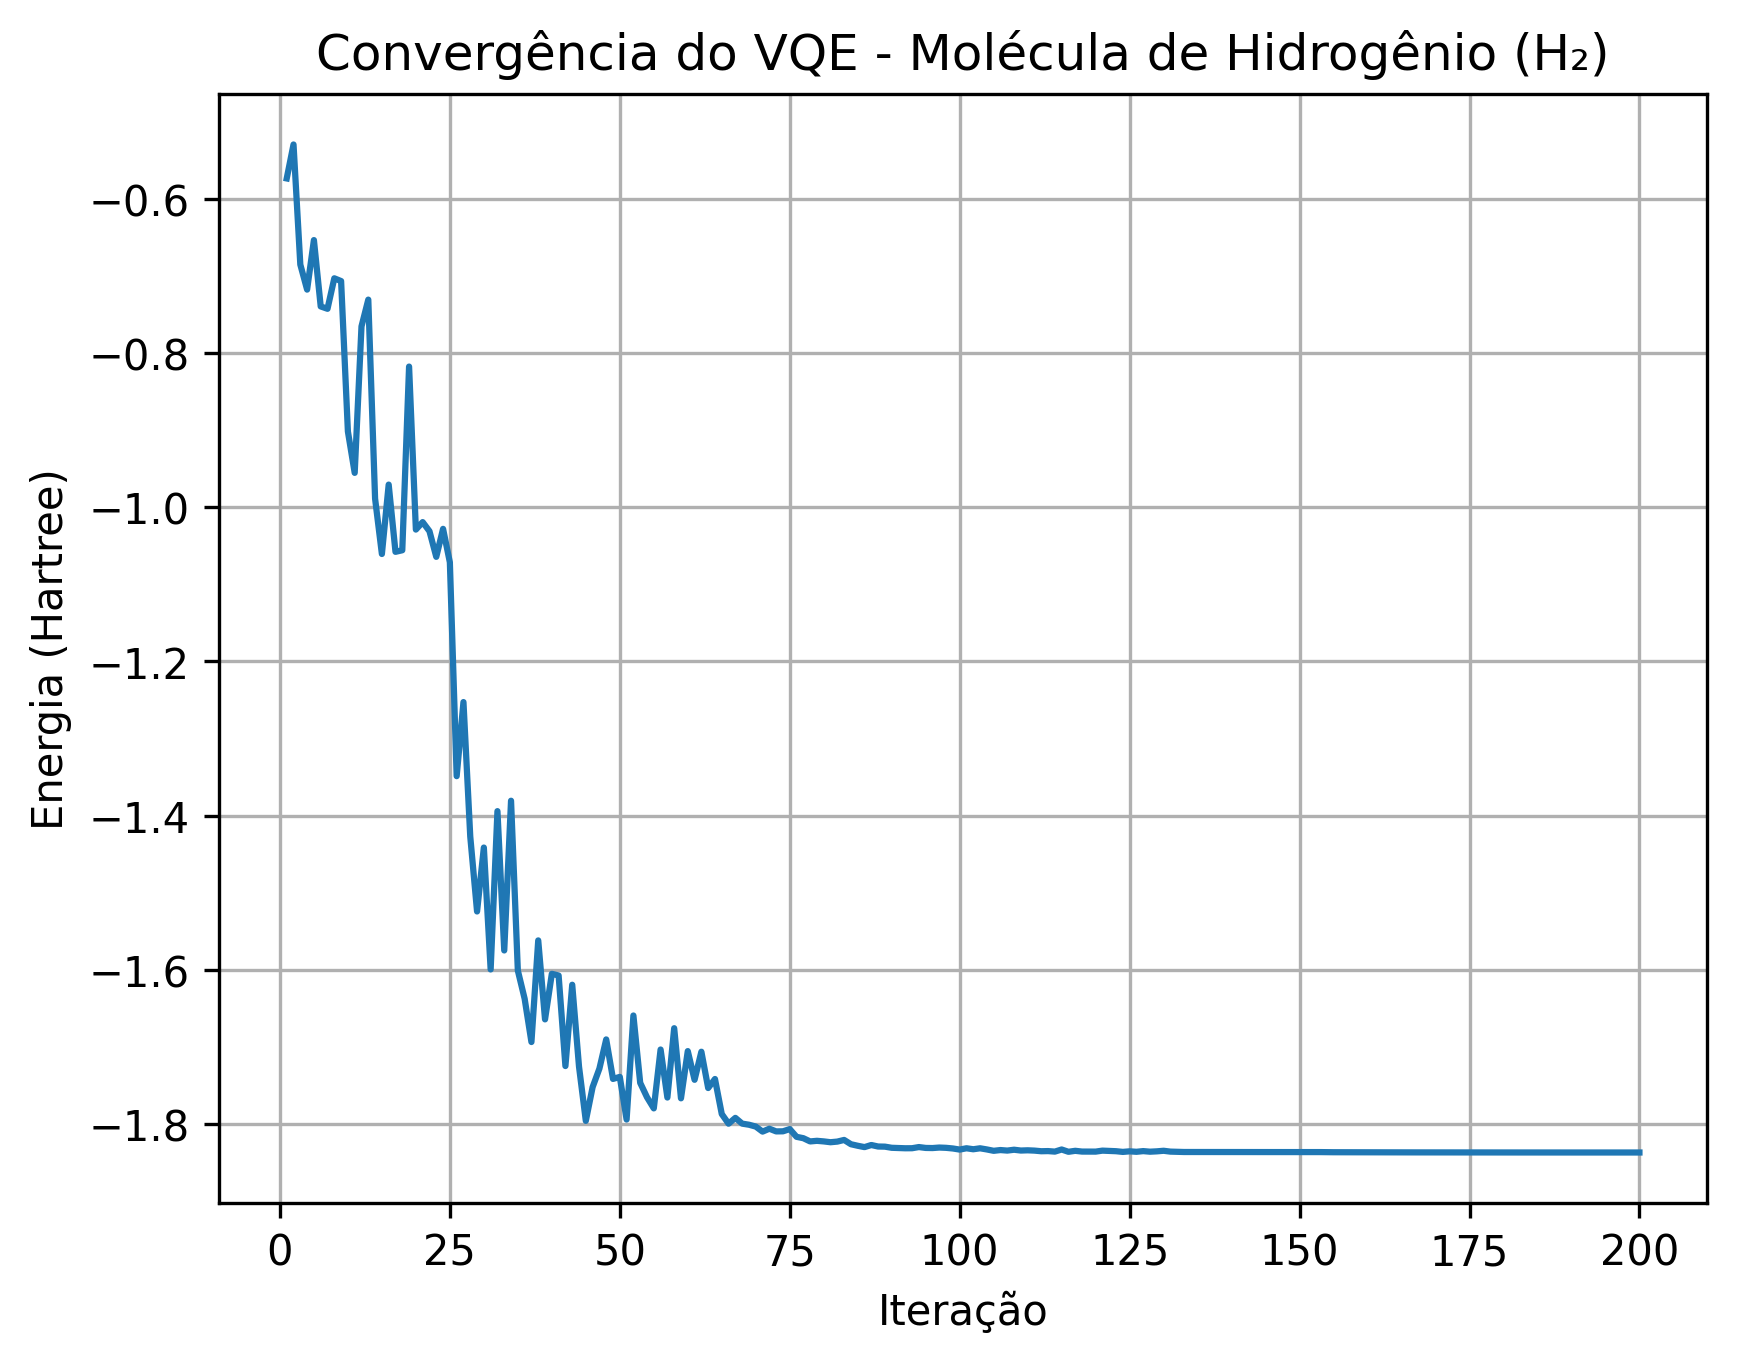
\includegraphics[width=0.6\textwidth]{img/h2_convergence.png} 
\caption{Convergência da energia variacional ao 
longo das iterações do VQE para a molécula de hidrogênio. Fonte: elaboração 
própria (2026).} 
\label{fig:h2_convergence} 
\end{figure}

A partir desse ponto, as variações tornam-se pouco significativas,
indicando convergência efetiva do procedimento variacional.
O comportamento relativamente suave da curva sugere uma paisagem
de custo com estrutura simples e bem comportada, característica
esperada para sistemas de baixa dimensionalidade como o H$_2$,
que envolve número reduzido de qubits e parâmetros variacionais.
Esse resultado evidencia a capacidade do VQE de reproduzir com
alta precisão a energia fundamental de sistemas moleculares
simples no regime NISQ, validando a implementação adotada.

O contraste com o comportamento observado para o LiH, discutido na
subseção seguinte, reforça o impacto do aumento da complexidade
eletrônica sobre a dinâmica de otimização variacional.

\subsection{Hidreto de Lítio (LiH)}

Para o sistema LiH, observou-se comportamento significativamente distinto
em comparação ao H$_2$. A energia variacional obtida foi 
$E_{\text{VQE}} = -7,9576$ $E_h$, enquanto o valor de referência
calculado por diagonalização exata foi 
$E_{\text{FCI}} = -8,8745$ $E_h$, resultando em erro absoluto
da ordem de $9,17 \times 10^{-1}$ $E_h$, aproximadamente 10,3\%
em termos relativos.

A Figura~\ref{fig:lih_convergence} evidencia um processo de otimização
marcado por oscilações significativas ao longo das iterações.
Diferentemente do comportamento observado para o H$_2$, o LiH não
apresenta convergência monotônica nem estabilização clara em torno
de um mínimo bem definido. Observa-se uma redução abrupta da energia
por volta da iteração 70, seguida de uma região prolongada de
flutuações de magnitude considerável.

\begin{figure}[H] 
\centering 
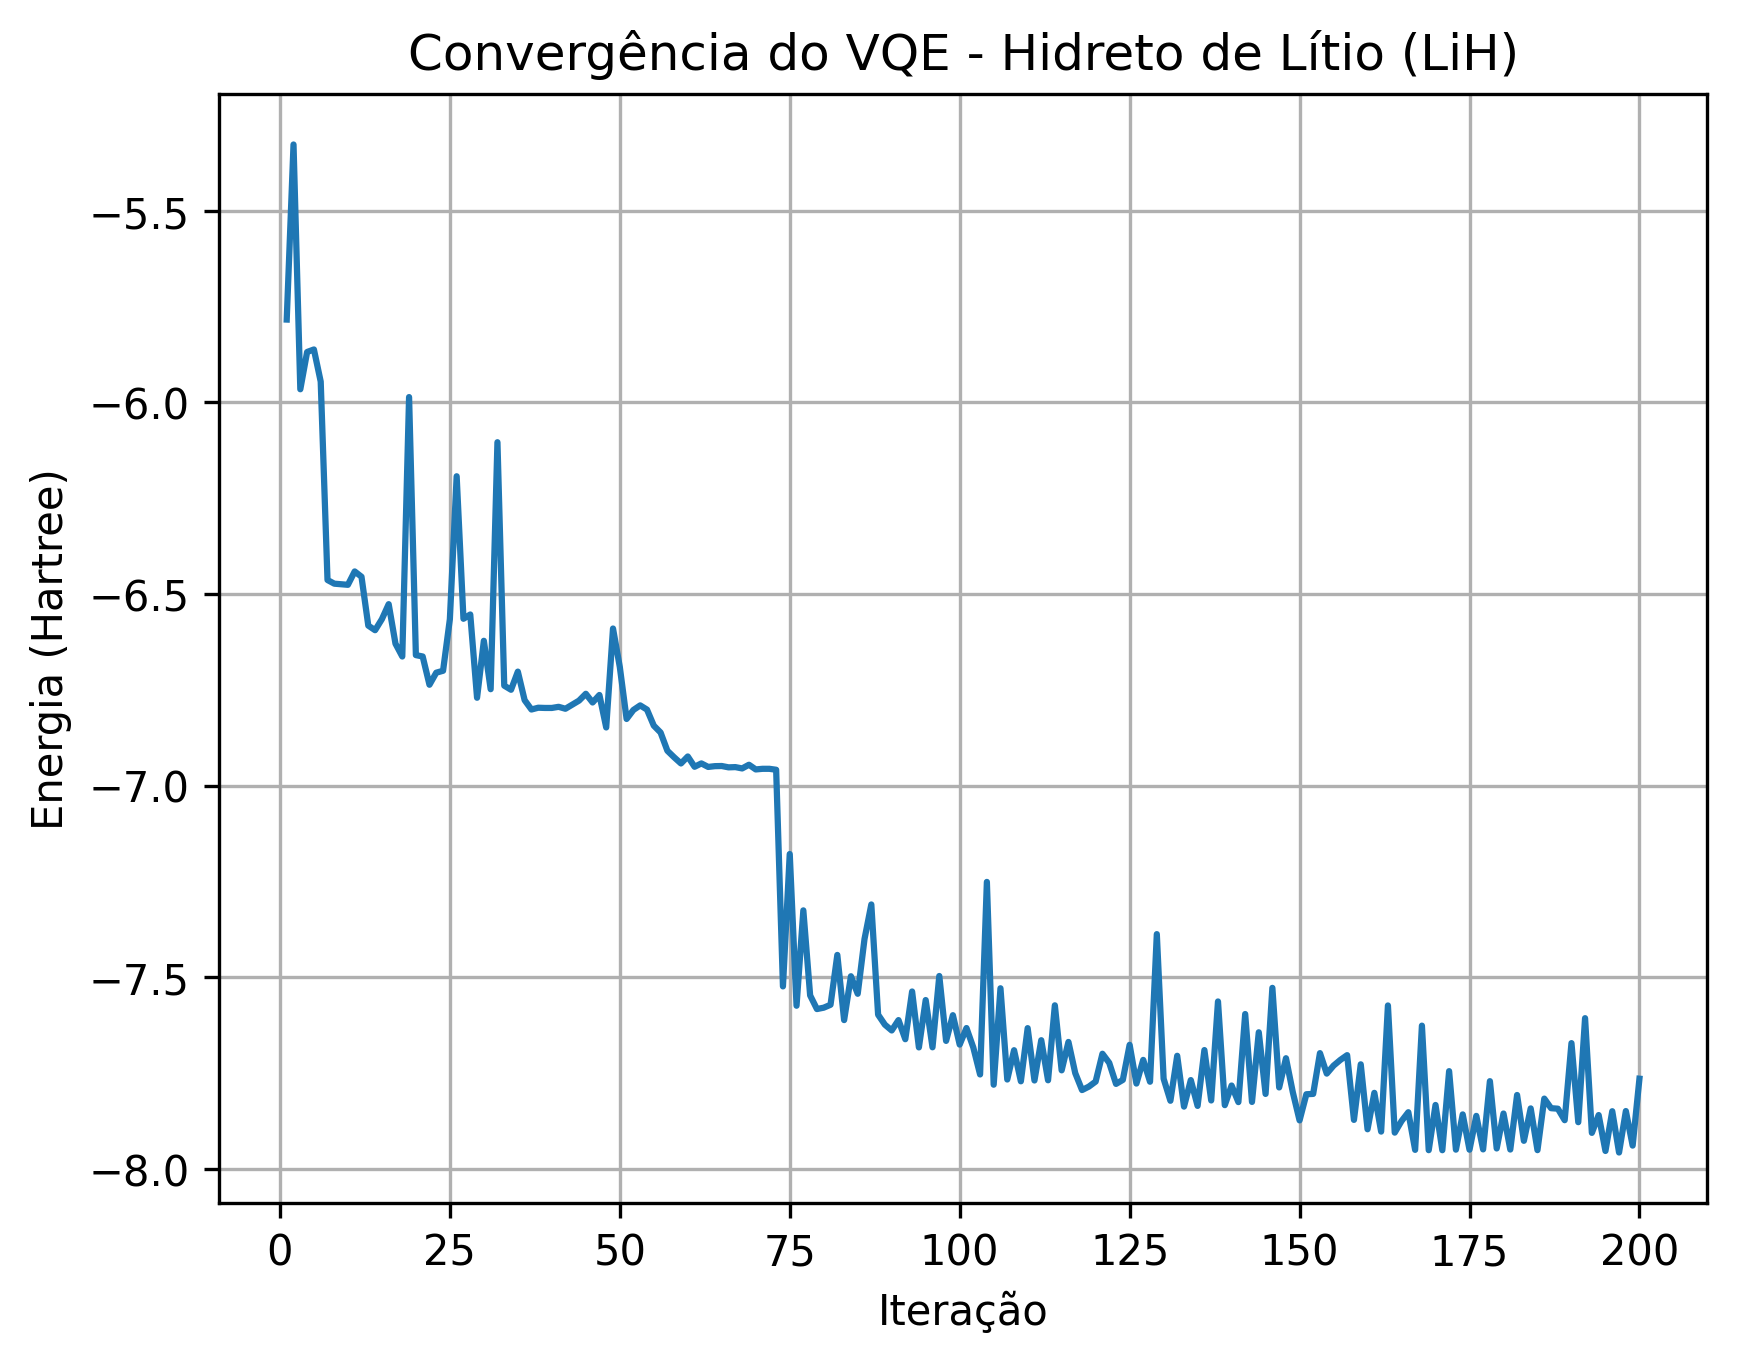
\includegraphics[width=0.6\textwidth]{img/lih_convergence.png} 
\caption{Convergência da energia variacional ao 
longo das iterações do VQE para a molécula de hidreto de lítio. Fonte: 
elaboração própria (2026).} 
\label{fig:lih_convergence} 
\end{figure}

Esse comportamento sugere uma paisagem variacional de maior
complexidade, possivelmente caracterizada por múltiplos mínimos
locais e regiões de curvatura irregular. O aumento do número de
qubits e parâmetros variacionais amplia a dimensionalidade do
espaço de busca, tornando o processo de otimização mais sensível
à escolha do \textit{ansatz} e à estratégia do otimizador clássico.

Além disso, a maior correlação eletrônica presente no LiH exige
maior expressividade do circuito variacional. O \textit{ansatz}
\textit{hardware-efficient} adotado, embora adequado para o regime NISQ
por sua baixa profundidade, pode não possuir capacidade suficiente
para capturar integralmente a estrutura eletrônica do sistema,
limitando a aproximação ao valor FCI.
A presença de oscilações persistentes também pode indicar que o
otimizador COBYLA, por ser livre de derivadas, realiza atualizações
com base em aproximações lineares locais que podem não refletir
adequadamente a geometria global da função custo em espaços de
maior dimensionalidade.

Portanto, os resultados obtidos para o LiH evidenciam, de forma
quantitativa e qualitativa, os desafios de escalabilidade do VQE
em sistemas moleculares mais complexos, destacando a necessidade
de estratégias mais expressivas ou técnicas de otimização mais
robustas para alcançar maior precisão.
Comparativamente, observa-se que o desempenho do VQE degrada à medida que
a complexidade molecular aumenta, evidenciando um dos principais desafios
da era NISQ: equilibrar profundidade de circuito, número de parâmetros e
capacidade expressiva sob restrições de recursos computacionais.
Os resultados obtidos, portanto, não apenas validam o funcionamento do
algoritmo em sistemas simples, mas também evidenciam, de forma quantitativa,
os desafios de escalabilidade inerentes à simulação variacional de sistemas
químicos mais complexos.
